\documentclass[11pt,a4paper,dvipsnames]{article}
\usepackage[margin=2.5cm]{geometry}
\usepackage{iohk}
\usepackage{microtype}
\usepackage{mathpazo} % nice fonts
\usepackage{amsmath}
\usepackage{amssymb}
\usepackage{amsthm}
\usepackage{latexsym}
\usepackage{mathtools}
\usepackage{subcaption}
\usepackage{stmaryrd}
\usepackage{extarrows}
\usepackage{slashed}
\usepackage[colon]{natbib}
\usepackage[unicode=true,pdftex,pdfa,colorlinks=true]{hyperref}
\usepackage{xcolor}
\usepackage[capitalise,noabbrev,nameinlink]{cleveref}
\usepackage{float}
\floatstyle{boxed}
\restylefloat{figure}
\usepackage{tikz}

%%
%% Package `semantic` can be used for writing inference rules.
%%
\usepackage{semantic}
%% Setup for the semantic package
\setpremisesspace{20pt}

\newcommand{\unitInterval}{\ensuremath{[0,~1]}}
\newcommand{\nonnegReals}{\ensuremath{[0,~\infty)}}
\newcommand{\posReals}{\ensuremath{(0,~\infty)}}

\theoremstyle{definition}
\newtheorem{definition}{Definition}[section]

\theoremstyle{definition}
\newtheorem{property}{Property}[section]

\begin{document}

\hypersetup{
  pdftitle={A Specification of the Non-Integral Calculations in the Ledger},
  breaklinks=true,
  bookmarks=true,
  colorlinks=false,
  linkcolor={blue},
  citecolor={blue},
  urlcolor={blue},
  linkbordercolor={white},
  citebordercolor={white},
  urlbordercolor={white}
}

\title{A Specification of the Non-Integral Calculations in the Ledger}

\author{Matthias G\"udemann  \\ {\small \texttt{matthias.gudemann@iohk.io}}}

%\date{}

\maketitle

\begin{abstract}
  This document defines a way to exactly calculate non-integral calculations in
  the ledger for Shelley which use elementary mathematical functions. The main
  objective is to give an unambiguous specification that gives the same results,
  independent of the architecture or programming language. The goal is to
  prevent chain forks because of slight differences in calculated results.
\end{abstract}

\tableofcontents
\listoffigures

\section{Introduction}
\label{sec:introduction}

The Shelley specification~\cite{shelley_spec} and the Ouroboros
protocol~\cite{ouroboros} use non-integral calculations. Most can be done in an
exact way using rational numbers and arbitrary precision integers which are
available in most programming languages or via external libraries.~\footnote{The
  most widely used library is the GNU multi-precision library (GMP)}

There are also instances where elementary functions are used which cannot be
represented as rational numbers and therefore require a different
treatment. This includes using the exponential function
$e^{x}, x \in \mathbb{R}$ to calculate a decay and non-integral exponentiation
$x^{y}, x, y \in \mathbb{R}$.

\section{Problem Description}
\label{sec:problem-description}

The calculations that involve elementary functions are concerned with decay of
the value to refund from a deposit, calculation of the pool reward via the
moving average and the leader election probability.

In all these cases, it is important that all distributed nodes calculate the
same values, else here might be a disagreement what to include in the blockchain
and forks might result. In the case of a single implementation, this will not be
a problem, as only one result is possible, but in the case of multiple
implementations, this can become an issue. As Cardano is striving to be a
specification defined cryptocurrency, we need an exact specification of how to
achieve this, allowing for independent implementations with the same behavior.

\section{Implementation Possibilities}
\label{sec:impl-poss}

There are three main different possibilities to implement non-integral
calculations. In Haskell, we can use typeclasses to design generic algorithms
which can handle different backends. Each back-end has its advantages and
disadvantages.

\subsection{IEEE~754 Floating Point}
\label{sec:ieee-754-floating}

A straight-forward approach is to use IEEE~754 floating-point arithmetic which
is generally supported by all relevant programming languages and CPU
architectures.

The basic arithmetic operations of IEEE~754 floating-point are well specified,
and they are very efficient due to direct HW implementation.

Double precision floating-point provides 53 bits (~15.99 decimal digits) of
precision which is slightly below the required precision to represent the
fraction of 1 lovelace, as there are $4.5\cdot10^{16}$ of them. Also, the
required elementary functions are not standardized and there can be differences
in different implementations. It is also worth noting that some architectures
provide excess precision~\footnote{The original x87 provided 80 bit
  floating-point}, which can result in slight differences in results. There
exist programming languages, e.g., D, which make use of this by default. Many
languages support excess precision but default to IEEE~754 64 bits, in
particular on amd64 most make use of SSE floating-point arithmetic. Another
source problems can be different rounding modes which some programming languages
allow changing, e.g., C, but others do not, e.g., Haskell.

\subsection{Rational Numbers}
\label{sec:rational-numbers}

Rational numbers can be implemented on top of exact arbitrary precision integral
arithmetic. Effectively one uses \emph{gcd} calculation to normalize the results
after each basic operation. This allows for arbitrary precise approximation of
all real numbers, but may also incur arbitrary long numerators or denominators.

These arbitrarily long numerators and denominators incur
non-predictable~\footnote{potentially > 1s for basic arithmetic operations}
run-time.

\subsection{Fixed Point Arithmetic}
\label{sec:fixed-point-arithm}

An alternative approach is to use fixed point arithmetic based on exact integers
where a proportion of the integer is used as fractional part. This prevents the
problem with using fully rational arithmetic which can get very inefficient and
allows to define the desired number of decimal digits.

As it is implemented purely in SW on top of exact integer arithmetic, on the one
hand it is less efficient than IEEE~754, on the other hand it can be made to
behave equivalently in different implementations.

The basic idea is the following: for $n$ decimal digits of precision, multiply
each integral value with $10^{n}$ and take this into account in the basic
operations. To use in the case of Cardano, this would mean using $n=17$ to
support the required 17 digits of precision to track each possible stake
fraction.

\subsection{Conclusion}
\label{sec:summary}

For the Cardano cryptocurrency, the approach based on fixed point arithmetic
seems to be the best adapted one. It allows for the desired precision and can be
implemented in an equivalent way, because it uses exact integer
arithmetic.~\footnote{There already exist two implementations, Haskell and C.}
While the fixed-point approach is less efficient than IEEE~754, using partial
pre-computation will be possible to speed it up in the case where the base of an
exponentiation is a constant.

\section{Approximation Algorithms}
\label{sec:algorithms}

The elementary functions required in the ledger are the exponential function and
the exponentiation. Exponentiation $x^{y}$ of arbitrary real numbers is
calculated via the identity: $x^{y}= \exp({\ln(x^{y})}) = \exp(y\cdot
\ln(x))$. This means we do need approximation schemes for $\exp(x)$ and
$\ln(x)$.

There exist two main approaches for approximation: Taylor / MacLaurin series and
continued fractions. Both require only basic arithmetic operations and allow for
iterative approximation, i.e., constructing a sequence of $x_{0},x_{1},\ldots
x_{n}$ where each $x_{i}$ is a better approximation for the desired value.

\subsection{Taylor Series}
\label{sec:taylor-series}

A Taylor series defines an infinite series that approximates an infinitely often
differentiable function around a point $a$. It does have the following general
form for a function $f$:

\begin{equation*}
  Tf(x; a) := \sum_{n=0}^{\infty}\frac{f^{(n)}(a)}{n!}
  {\left(
    x - a
  \right)}^{n}
\end{equation*}

Most often one develops the Taylor series at $a=0$ which is also called
MacLaurin series and uses a truncated, finite polynomial for the function
approximation as follows:

\begin{equation*}
  x_{m} := \sum_{n=0}^{m}\frac{f^{(n)}(0)}{n!} x^{n}
\end{equation*}

Using the above, one approximates the exponential function using Taylor series
as

\begin{equation*}
  \exp(x) := \sum_{n=0}^{\infty}\frac{x^{n}}{n!}
\end{equation*}

and the natural logarithm as

\begin{equation*}
  \ln(x) := \sum_{n=1}^{\infty}\frac{(-1)^{n+1}}{n}
    {\left(
        x - 1
    \right)}^{n}
\end{equation*}

\subsection{Continued Fractions}
\label{sec:continued-fractions}

Continued fractions are a way to represent a number as the sum of its integral
part and the reciprocal of another number. The most general form looks like
this:

\begin{equation*}
  b_{0} + \cfrac{a_{1}}{b_{1} + \cfrac{a_{2}}{b_{2}  + \cfrac{a_{3}}{\ddots}}}
\end{equation*}

The covergents $x_{i} = \frac{A_{i}}{B_{i}}$ are computed via the following
recursion:

\begin{align*}
  A_{-1} & :=  1 \\
  A_{0} & :=  b_{0} \\
  B_{-1} & :=  0 \\
  B_{0} & := 1 \\
  A_{n} & :=  b_{n}\cdot A_{n-1} + a_{n}\cdot A_{n-2} \\
  B_{n} & :=  b_{n}\cdot B_{n-1} + a_{n}\cdot B_{n-2}
\end{align*}

For the exponential function $\exp(x)$, the sequences of $a_{i}$ and $b_{i}$ are
the following:

\begin{align*}
  \sigma(a_{i}) & := 1 \cdot x, -1 \cdot x, -2 \cdot x, \ldots \\
  \sigma(b_{i}) & := 1, 2 + x, 3 + x, \ldots
\end{align*}

For the natural logarithm $\ln(x+1)$, the sequences of $a_{i}$ and $b_{i}$ are
the following:

\begin{align*}
  \sigma(a_{i}) & := 1^{2}\cdot x, 1^{2}\cdot x, 2^{2}\cdot x, 2^{2}\cdot x, 3^{2}\cdot
          x, 3^{2}\cdot x, \ldots\\
  \sigma(b_{i}) & := 1, 2, 3, \ldots
\end{align*}

\subsection{Scaling}
\label{sec:scaling}

Both Taylor series and continued fractions do not converge for arbitrary input
values, their convergence radius is limited. Therefore we apply scaling before
we do the approximation, using the mathematical properties of $\exp$ and $\ln$
to get the correct results.

To calculate the exponential functions, we scale $x$ in such a way that
$x \in [0; 1]$ via:

\begin{equation*}
  \exp(x) = \exp
  \left(
    \frac{x}{n}\cdot n
  \right) =
  {\left(
      \exp{
        \left(
          \frac{x}{n}
        \right)}
    \right)}^{n}, \text{ with } n := \lceil x \rceil
\end{equation*}

For the natural logarithm, we calculate $n$ in such a way that
$\exp(n) \leq x < \exp(n+1)$ and use this as follows:

\begin{equation*}
  \ln(x) = \ln
  \left(
    \exp(n) \cdot \frac{x}{\exp(n)}
  \right) = \ln(\exp(n)) + \ln
  \left(
    \frac{x}{\exp(n)}
  \right) = n + \ln
  \left(
    \frac{x}{\exp(n)}
  \right)
\end{equation*}

which guarantees that $\frac{x}{\exp(n)}$ is in the interval $[1; e]$ which lies
in the convergence radius of the approximation schemes.

\subsection{Convergence}
\label{sec:convergence}

Experimental results have shown that continued fractions have a better
convergence speed, in particular for the natural logarithm.

\begin{figure}[ht]
  \centering
    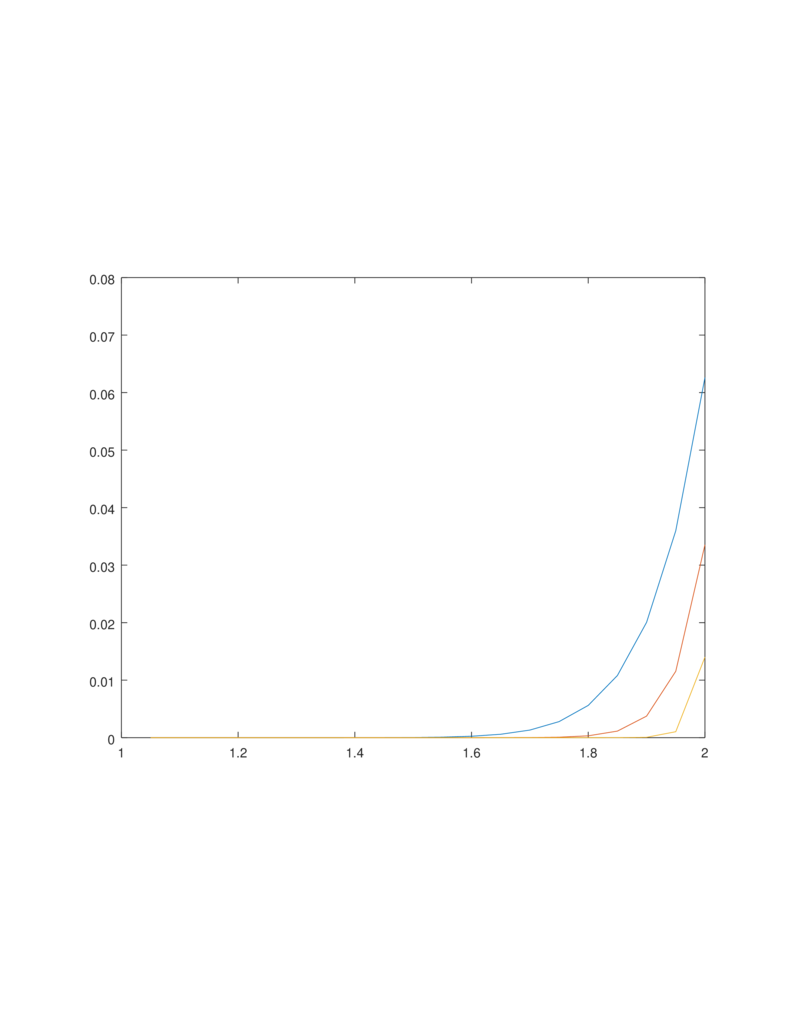
\includegraphics[width=\textwidth]{ln_taylor}
  \caption{Relative Error for Taylor Series Approximation of  $\ln$}
  \label{fig:ln-approx-taylor}
\end{figure}

\begin{figure}[ht]
  \centering
    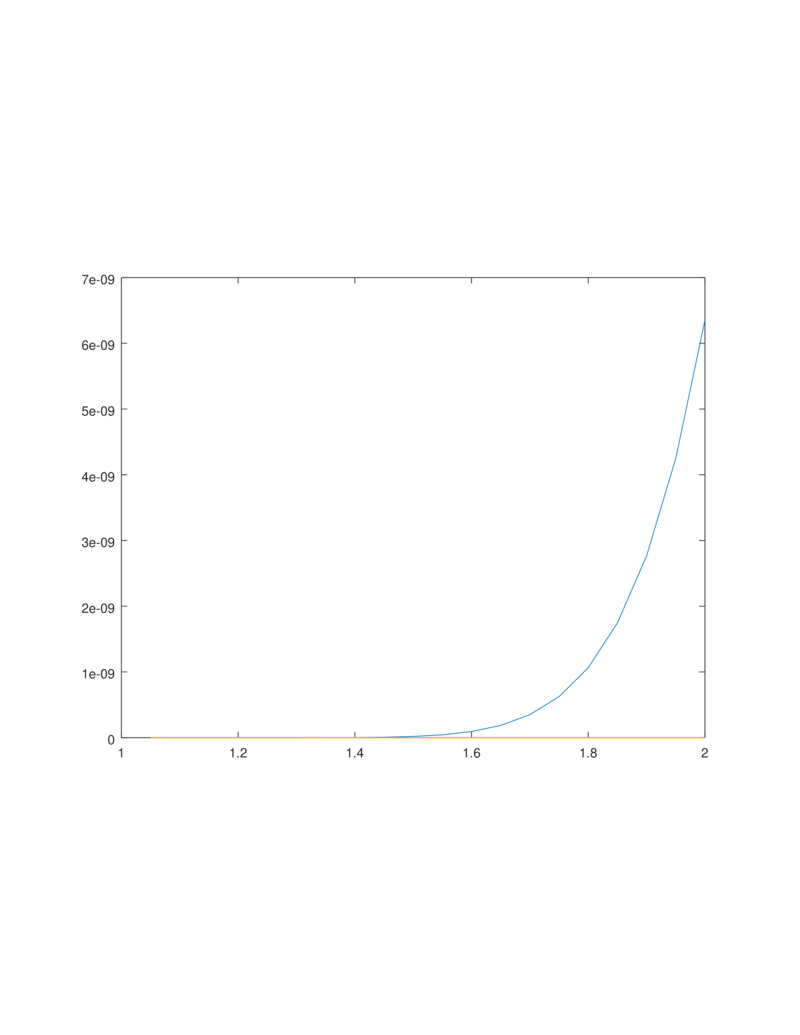
\includegraphics[width=\textwidth]{ln_cf}
  \caption{Relative Error for Continued Fraction Approximation of  $\ln$}
  \label{fig:ln-approx-cf}
\end{figure}

Figure~\ref{fig:ln-approx-taylor} shows the relative approximation error for
$\ln$ with 10, 20, and 50 iterations using a Taylor
series. Figure~\ref{fig:ln-approx-cf} shows the relative approximation error for
10, 20, and 50 iterations using continued fractions. In this case, the error of
the continued fraction approach is multiple orders of magnitude lower for the
same number of iterations.

\begin{figure}[ht]
  \centering
    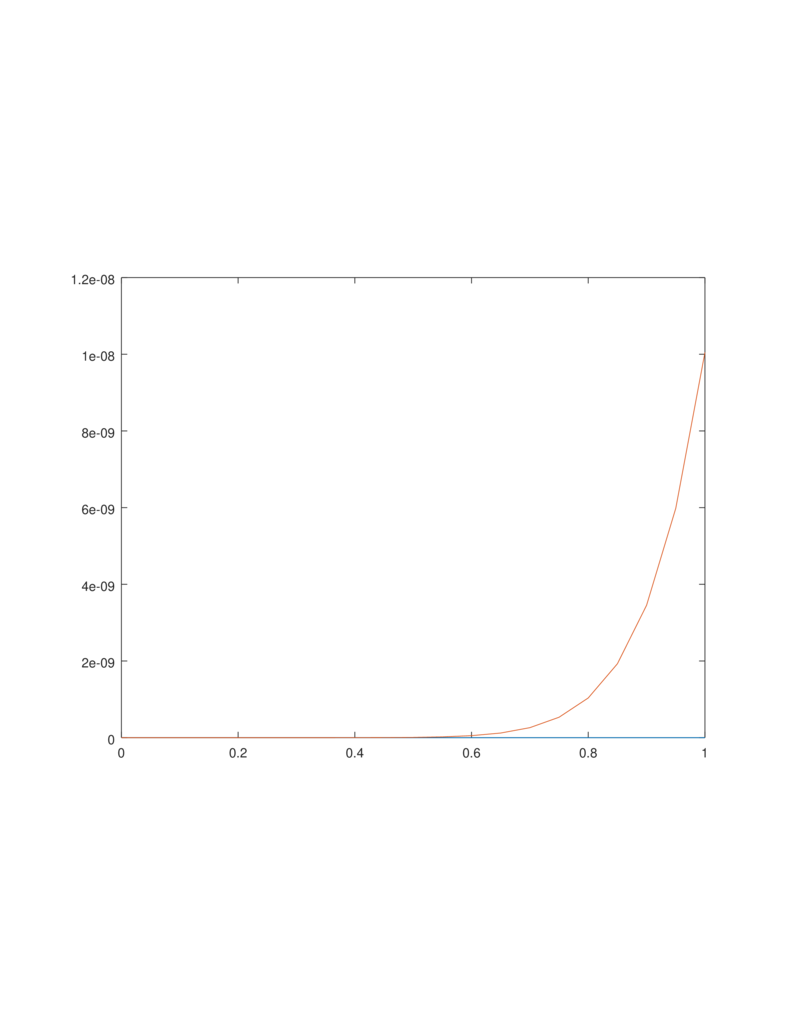
\includegraphics[width=\textwidth]{taylor_exp}
  \caption{Relative Error for Taylor Series Approximation of  $\exp$}
  \label{fig:exp-approx-taylor}
\end{figure}

\begin{figure}[ht]
  \centering
    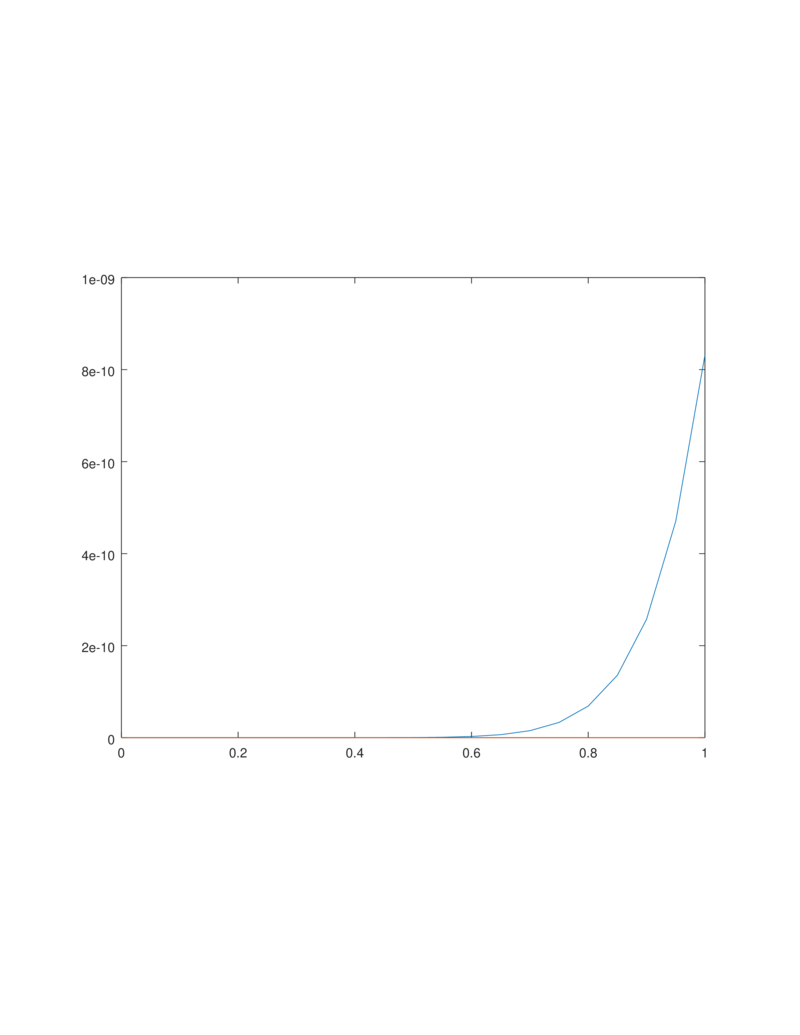
\includegraphics[width=\textwidth]{cf_exp}
  \caption{Relative Error for Continued Fraction Approximation of  $\exp$}
  \label{fig:exp-approx-cf}
\end{figure}

Figure~\ref{fig:exp-approx-taylor} shows the relative approximation error of 10
and 20 iteration using a Taylor series approach. Figure~\ref{fig:exp-approx-cf}
shows the relative error of 10 and 20 iterations using continued fractions. In
this case the error of continued fractions is around one order of magnitude
lower for the same number of iterations.

\subsection{Conclusion}
\label{sec:conclusion}

From these experiments one can conclude that the convergence speed is higher for
continued fractions, in particular for the natural logarithm. On the other hand,
timing analysis showed that due to the simpler calculation per iteration of
Taylor series, the exponential function can be approximated more efficiently
using that approach. Therefore we decided to use both, Taylor series for $\exp$
and continued fractions for $\ln$.

To decide when the approximation has enough precision, we use the following
criterion for two succeeding approximations $x_{n}, x_{n+1}$:
\begin{equation*}
  \vert x_{n} - x_{n+1}\vert < \epsilon
\end{equation*}

Therefore both approximation schemes result in the same precision.

\section{Reference Implementation}
\label{sec:refer-impl}

The continued fraction approach using fixed point arithmetic has been
implemented in Haskell and in C using the GNU multi-precision
library~\footnote{\url{https://gmplib.org}}.

For the Haskell version there are Quickcheck property-based tests that validate
mathematical consistency of the laws for $\ln$ and $\exp$.

For both the C and the Haskell version there exists a test program that reads
two fixed pointed numbers with 34 decimal digits of precision and calculates
$x^{y}$ from them. This has been used to validate the two different
implementations for 20.000.000 randomly generated testcases where $x$ and $y$
were drawn uniformly from the interval $[0.1; 100.1]$, which showed that all
results were exactly the same for all 34 decimal digits.

The important aspect to get equivalent results is using the same approach to
rounding after a division. In particular we use rounding to $-\infty$.

\section{Optimisations for Specific Use-Cases}
\label{sec:optim-spec-use}

One use case for non-integral calculations in Shelley is the calculation of the
probability of being a slot leader. This calculation has to be done every 2s
locally for each potential slot leader. It also needs to be done in order to
validate a block (to make sure that the block producer actually had the right to
do so).

More precisely, one has to check whether for a given $p$, $\sigma$ and a
constant (at least for one epoch) $f$ the following inequality holds:

\begin{equation*}
  p < 1 - {(1 - f)}^{\sigma}
\end{equation*}

As $1-f$ is considered to be constant, and because ${(1-f)}^{\sigma}$ is equal
to $\exp(\sigma\cdot\ln(1-f))$, we can pre-compute the value of $\ln(1-f)$ once
and use it for every following computation.

Setting $c:= \ln(1 - f)$ and using $q := 1 - p$ we get the following:

\begin{equation*}
  \begin{array}[h]{ccc}
    & p < 1 - \exp(\sigma \cdot c) & \\
    \Leftrightarrow & \exp(\sigma \cdot c) < 1 - p & (\textrm{c is negative})\\
    \Leftrightarrow & \frac{1}{\exp(-\sigma \cdot c)} < q & \\
    \Leftrightarrow & \frac{1}{q} < \exp(-\sigma \cdot c) &
  \end{array}
\end{equation*}

The term $\exp(-\sigma \cdot c)$ can be computed using the Taylor series as
described in Section~\ref{sec:taylor-series}.

As the relevant information is not the result of the calculation, but whether
the given $p$ is less than or greater than this value, one can also optimize
further. Using the Lagrange remainder to estimate the error, it is possible to
only compute as many iterations as necessary to get the desired information.

\begin{equation*}
    T \exp(x; a) := \sum_{n=0}^{\infty}\frac{x^{n}}{n!} =
    \sum_{n=0}^k\frac{x^{n}}{n!} + R_{k}(x)
\end{equation*}

Where using an upper bound $M$ on the domain of $x$, the remainder (or error
term) $R_{k}(x)$ can be estimated as follows:

\begin{equation*}
  R_{k}(x) \leq \vert M \cdot \frac{x^{k+1}}{(k+1)!}\vert
\end{equation*}

For the use-case of the leader election, a good integral bound for the error
estimation is the maximal value of $\vert\ln(1 - f)\vert\leq M$ for
$f \in [0, 0.95]$ is $M = 3$. For any larger value of $f$, a different value
would have to be chosen. The current value for $f$ is $0.1$.

In general, for this use case one can easily estimate $M$, as the smallest
integer larger than the exponential function evaluated at the upper bound of the
interval of the domain of $x$. For each partial sum $\Sigma_{k}$, one can then
test whether $p$ is greater than $\Sigma_k + \vert R_{k}(x) \vert$ or less than
$\Sigma_k - \vert R_{k}(x)\vert$ to decide whether one can stop at an early
iteration.

\begin{figure}[ht]
  \centering
  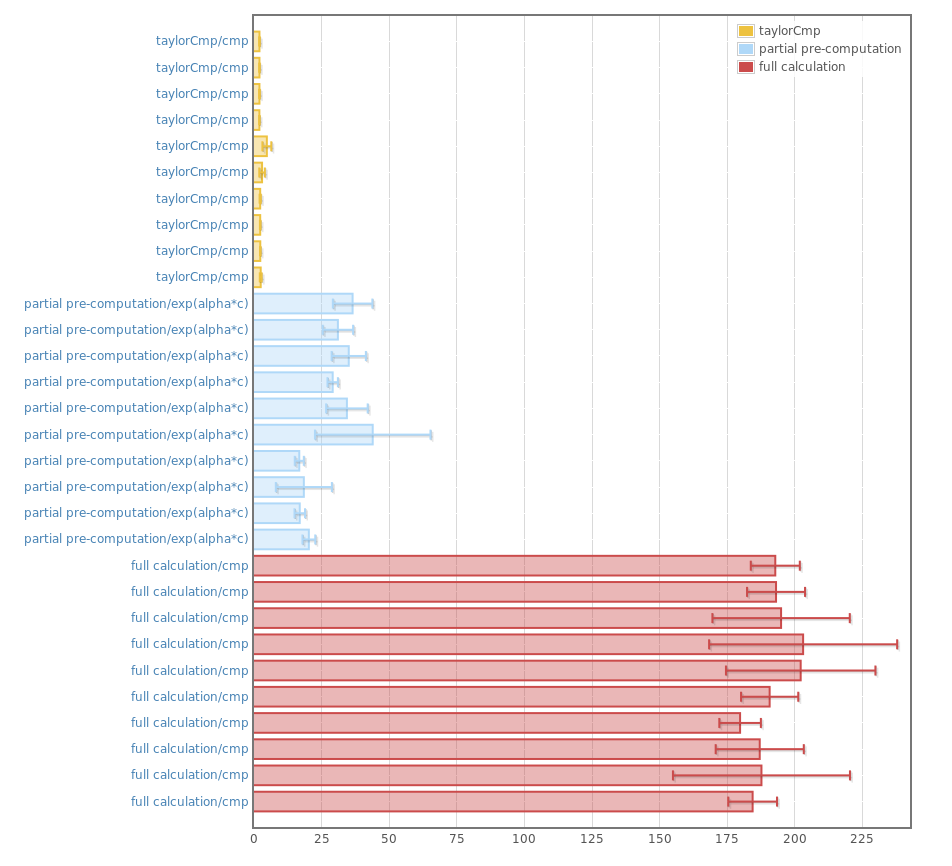
\includegraphics[width=0.75\textwidth]{haskell.png}
  \caption{Benchmark Results for the Haskell Implementation}
  \label{fig:haskell-optimization-results}
\end{figure}

Figure~\ref{fig:haskell-optimization-results} shows the benchmark results for
test data using the Haskell implementation. The lower (red) results show the
run-time (in $\mu s$) for the naive, full computation. The middle (blue) part
shows the run-time using a partial pre-computation of $\ln (1-f)$ for the
exponentiation. The upper (yellow) part shows the run-time using the proposed
optimization. For the 10 data points, the first 5 succeed in the leader
election, the remaining 5 do not.

\addcontentsline{toc}{section}{References}
\bibliographystyle{plainnat}
\bibliography{references}

\end{document}

%%% Local Variables:
%%% mode: latex
%%% TeX-master: t
%%% End:
